% Seminar paper for High-Performance Computing with FPGAs (SS2018)
% Gaurav Kumar Singh <gauravks@mail.uni-paderborn.de>
%
% based on a template by Holger Karl, (c) 2001

\documentclass[12pt,twoside]{article}
\usepackage{url}


%%%%%%%%%%%%%%%%%%%%%%%%%%%%%%%%%%%%%%%%%%%%%%%%%%%%%%%%%%%%%%%%%%%%%%%%%%%%%%
%%%%%%%%% configure these settings and you are good to go %%%%%%%%%%%%%%%%%%%%
%%%%%%%%%%%%%%%%%%%%%%%%%%%%%%%%%%%%%%%%%%%%%%%%%%%%%%%%%%%%%%%%%%%%%%%%%%%%%%
\newcommand{\participant}{Gaurav Kumar Singh}
\newcommand{\affiliation}{Paderborn University}
\urldef{\emailaddress}\url{gauravks@mail.uni-paderborn.de}
\newcommand{\topic}{Accelerating Bioinformatic applications using FPGA based HPC system}


%%%%%%%%%%%%%%%%%%%%%%%%%%%%%%%%%%%%%%%%%%%%%%%%%%%%%%%%%%%%%%%%%%%%%%%%%%%%%%
%%%%%%%%% don't make any other changes in the following   %%%%%%%%%%%%%%%%%%%%
%%%%%%%%% preamble unless you know what you are doing     %%%%%%%%%%%%%%%%%%%%
%%%%%%%%%%%%%%%%%%%%%%%%%%%%%%%%%%%%%%%%%%%%%%%%%%%%%%%%%%%%%%%%%%%%%%%%%%%%%%

\usepackage[english]{babel}
\usepackage[T1]{fontenc}
\usepackage[utf8]{inputenc}
\usepackage{times}
\RequirePackage[style=ieee,doi=true,isbn=false,url=false,mincitenames=1,maxcitenames=3,minbibnames=10,maxbibnames=10]{biblatex}
\usepackage{geometry}
\geometry{a4paper,body={15cm,22cm}}
\RequirePackage{xpatch}
\xpatchbibmacro{textcite}{\addspace}{\addnbspace}{}{}
\xpatchbibmacro{Textcite}{\addspace}{\addnbspace}{}{}
\usepackage{amsmath}
\usepackage{multirow}
\usepackage{graphicx}
\usepackage{paralist}
\usepackage{fancyhdr}
\usepackage{cleveref}
\usepackage[font=footnotesize,labelfont=bf]{caption}
\RequirePackage[margin=0cm]{subfig}
\bibliography{references}
\pagestyle{fancy}
\fancyhead{}
\fancyhead[LE]{ \slshape \participant}
\fancyhead[LO]{}
\fancyhead[RE]{}
\fancyhead[RO]{ \slshape \topic}
\fancyfoot[C]{}

\begin{document}

\title{\topic}
\author{\Large{\participant}\\ \affiliation \\ {\small \emailaddress}}
\date{}
\maketitle
\thispagestyle{empty}

%%%%%%%%%%%%%%%%%%%%%%%%%%%%%%%%%%%%%%%%%%%%%%%%%%%%%%%%%%%%%%%%%%%%%%%%%%%%%%
%%%%%%%%% here starts the actual text                     %%%%%%%%%%%%%%%%%%%%
%%%%%%%%%%%%%%%%%%%%%%%%%%%%%%%%%%%%%%%%%%%%%%%%%%%%%%%%%%%%%%%%%%%%%%%%%%%%%%

% Abstract gives a brief summary of the main points of a paper:
\begin{abstract}

 The Human Genome project was marked as completed in the year 2003 which opened vast avenues 
 for research towards developing and enhancing Genomic analysis techniques. With such vast sequence
 database available, the Genomic research greatly relied on bioinformatics capabilities. Improvements
 to the computational speed were necessary to discover causes and treatments for various
 diseases faster. This has been a major driving factor to develop techniques to increase the processing
 capabilities of the existing algorithms, tools and techniques by utilizing advancements in computing.
 FPGA based acceleration presents very promising advantages, reducing processing times
 by huge factor compared to other CPU and GPU based techniques. Similarly, the introduction of high performance
 clusters to distribute the processing has already been used and shown to be effective for large sequence analysis.

 Combining these technologies together possess great benefits for speeding up the analysis of the huge databases further.
 This paper will present a heterogenous system which have been developed using different accelerators to
 speed up the genome analysis from and reduce time form years to days. Initially we look at bioinformatics application
 areas where  FPGA and HPC system are beneficial. Then the paper describes some of the algorithms which can be accelerated
 using FPGA and HPC in a heterogenous system. The last part presents a system and evaluation
 results in terms of speedup compared to existing systems and tools.

\end{abstract}

% the actual content, usually separated over a number of sections
% each section is assigned a label, in order to be able to put a
% crossreference to it

\section{Introduction}
\label{sec:introduction}

Humans quest to understand the basic biological processes lead to development of research areas such as
biochemistry and biotechnology. Multiple decades of research in the biological molecules helped us in
understanding the existence DNA and genome which defines how a living organism behaves and exist.
On the other hand the advancement in computer technologies and increased use of them in healthcare, biomedical
and computational biological research has helped find cure and medical treatments for many complex health
issues and save many lives over the years.

In efforts to increase the knowledge of genomes, the field of Bioinformatic was created. Bioinformatic majorly involves
the study of biological molecules (biomolecules) which build up the cells of the living organisms. As with the other biological fields,
bioinformatic aims at utilizing the capabilities of the computer science to build and analyse molecular sequences (genes) of DNA.
In this direction, The \emph{Human Genome Project}\footnote{\url{http://https://www.genome.gov/}}  was started in late 1990 and was
completed in 2003 successfully. "A 2.91-billion base pair (bp) consensus sequence of the euchromatic portion of
the human genome was generated by the whole-genome shotgun sequencing method"\cite{venter_sequence_2001}. This was a huge
step but also presented the problem of huge processing times for analysis of such a large database of genome for extracting any
useful information. The existing algorithms for database searches such as Smith-Waterman \cite{smith_identification_1981} based
on dynamic programming for local similarity estimation and heuristics based BLAST \cite{altschul_basic_1990} were limited by
high computation times. The main limiting factors at this point were the processing capabilities of the computing units
on which the algorithms were running.

Various methods in the past decades have evolved to provide higher computing and data processing capabilities for various application domain.
The earliest method being hardware acceleration provided by symmetric multiprocessing which allows distribution of computing to different processor
sharing a common memory. The next major acceleration achieved has been the development of high performance computing clusters (HPC).  HPC
system work by splitting and distributing the problem over multiple similar processing units popularly known as nodes. Each of the node,
consists of a high performance processor with multiple cores and sharing the same common memory. The nodes in the clusters are connected to
each other with high speed Ethernet connections for exchange of data and control information. Each node can be used to
process a sub-set of the data parallely decreasing the overall computing time for the problem. Due to such benefits, these techniques were
introduced for Bioinformatic algorithms to speed up processing time.
Implementation of the famous Smith-Waterman algorithm on HPC systems is presented in \cite{boukerche_parallel_2005,martins_multithreaded_2000}.
A various number of parallel implementation for BLAST such as mpiBLAST \cite{darling_design_2003} are available as well, which prove
to be more time efficient. \textcite{schmidt_massively_2002} showed how such improvements can be used to create a parallel system which
helps to speed up the molecular sequence analyse.

Another step in increasing the processing capabilities of the clusters was utilization of GPU. GPUs allow offloading
the vector based arithmetic operations for large datasets. They prove to be excellent accelerators for reducing
the processing time with large amount of data. \textcite{liu_cuda-blastp:_2011} have presented such a system which is capable of performing
10 times faster compared to serial versions of BLAST \cite{altschul_basic_1990}.

Though the parallel implementation with CPU and GPU help in achieving faster processing time, its heavily dependant
on the size of the cluster. Also the speedup highly depends on the size of the problem. These reasons
made researchers to look for areas for improving the execution times of the algorithm by using hardware based
accelerators by reducing processing time for each operation. This is where the FPGA has 
helped a lot by providing opportunities to implement the algorithms directly in the hardware. The flexibility
of FPGA based accelerators makes them very useful to design application specific acceleration hardware and
re-use them for different kinds of problems. Currently a lot of accelerators are available from which, the bioinformatic
community is benefiting. This paper would discuss some of these implementation and give an overview of how
such accelerators are integrated with the HPC clusters to build heterogenous systems which are used to
achieve very high processing speeds to reduce the time from days to hours for some bioinformatic application.

The rest of the paper is divided into 3 sections. Section 2 introduces the bioinformatic application domain giving
details of algorithms and tools popularly used. Section 3 will present the optimization techniques for genome
comparison by FPGA and heterogenous systems and the last section presents results achieved by such optimization
for some of the current systems.

\section {Bioinformatic and its applications}

Bioinformatic can be considered as an amalgamation of molecular biology and computer science.
As described by \textcite[chapter 8]{gokhale_reconfigurable_2010}, it mainly focuses on analysis
and management of biomolecular data to support research works for identifying causes of diseases and
specialized drug discovery. As mentioned in the introduction one of the most prominent success in
the field of Bioinformatics was completing sequencing the human genome. Apart from genome assembly
and analysis, bioinformatic also concentrates on protein classification and structure prediction,
gene prediction and phylogenetic prediction.

Genomic data is mainly build up from DNA or protein sequences. DNAs are build from a sequence of
nucleotide base pairs(bp). The four nucleotide molecules adenine (A), thymine (T), cytosine (C), and guanine (G)
form these base pairs and are always arranged such that adenine (A) pairs with thymine (T) and
cytosine (C) pairs with guanine (G). These bp can arrange in different ways and different lengths to build up the DNA
sequences. The DNA sequences form the gene, the entity known to be responsible for some specific functionality,
or the complete genome of the organism. The sequence of DNA are stored on computers as string containing only the
the alphabets A, T, C and G representing the respective nucleotide molecules. Similarly the protein molecules
are also represented by 20 \{A, C, D, E, F, G, H, I, K, L, M, N, P, Q, R, S, T, V, W, Y\} alphabets assigned
based on the ammino acids composition.

\textcite[chapter 2]{mount_bioinformatics:_2004} describes the complex DNA sequencing process which involves
extraction of the DNA fragments by using polymerase chain reaction (PCR) and tagging them for identification.
Genome sequencing involves a laborious process of generating smaller subclones of the original sequence and
then identifying overlaps to assemble the sequences. Small sequence are easy and cost effective to identify
and record but identification of the complete genome with similar techniques can be very costly. To reduce
the cost the small sequences are fed into the computer to create sequence databases using the string
representation of the bp and then computer programs are used to assemble them by identifying overlaps.
Genome databases collect such new sequences and provide them to researchers for analysis. The main
focus of the analysis is identification of similarity between genomes of different organisms and mapping
functions to the gene. Such similarities help to identify and build the divergence tree of species
through years of evolution. The gene mapping is also important to understand how the body behaves and can
be used to study effects of different chemicals during drug trials.

All of these studies require some form of string matching to compare or identify subsection from the huge
databases. As string comparison involved in the algorithms can be done with simple mathematical
operations over long operands, they can be easily mapped on simple circuits on the FPGA. As these
operations does not involve any complex floating point operations FPGA are suitable to speed up the
processing with dedicated hardware.

The rest of this section will explain the Bioinformatic application areas where FPGAs based accelerators
can be used to speed up the processing. Some of the algorithm will also be presented to understand there
functionality and usage in the bioinformatic domain.

\subsection{Application areas}

As highlighted earlier, the FPGAs can be a suitable target to accelerate the simple processing requirements
of the bioinformatic domain and speed up the processing by huge factor. In this subsection, some of the
application areas where FPGAs are suitable will be explained.

\subsubsection{Genome Assembly/sequencing}

Identification of the complete DNA sequence or the Genome of an organism has been one of the most common
application of bioinformatic from the early 1990. The identification of complete DNA sequence involves
forming small fragments of subclones of the large sequences and then re-arrange the fragments by comparing
the ends to find overlaps between the fragments\cite[Chapter 2, Genome sequencing]{mount_bioinformatics:_2004}.
This method is know as the shotgun sequencing and has been used to create the complete genomes of many organism
including human genome as shown in \cref{fig:sequence}.

\begin{figure}%
    \centering
    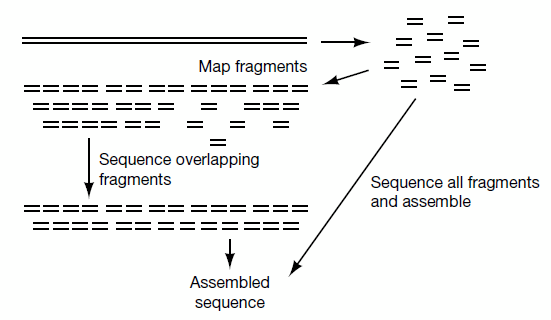
\includegraphics[width=0.8\textwidth]{fig/sequence}
    \caption{Sequencing process \cite[Figure 2.4]{mount_bioinformatics:_2004}}
    \label{fig:sequence}
\end{figure}

The main idea involved is comparison of overlap regions in the fragments to arrange them in the sequence. This
is mostly achieved in computers by using pairwise comparisons of the strings for the fragments and identifying
the similarities towards the end. Such comparison which mostly involve simple comparison operation of some
fixed number values can be easily implemented in FPGA with high accuracy.

\subsubsection{Gene prediction}

One of the important aspect of DNA sequencing to identify the sequences which perform a specific functionality
within the organism. Such sequences are called genes and an organisms genome can be divided into 100 of gene
segment, each of which can be mapped to some specific functionality. The functionality of the gene are identified
by predicting the sequences which encode some proteins molecule. Such sequences are identified by looking for
open reading frames (ORF) which are sequences of bp which contains a codon encoding one of the ammino acid.

Gene prediction algorithm use the known databases of ammino acid sequences to identify similar patterns in the
in the genome and tag them with the identified ammino acid. The ammino acid sequences are used to identify
the resulting protein structure and predict it by searching for similar ones on know organism genome. The searches
for gene prediction involve multiple databases and can be time consuming if whole database is required to be
searched element by element for accuracy. Accurate algorithm based on dynamic programming are available which
can perform the exhaustive search but to reduce the complexity of the search, heuristics based algorithms
such as BLAST \cite{altschul_basic_1990} are often used. Such algorithm can't guarantee mathematical accuracy
but are known to be good in the predictive search and reducing the search time.

FPGAs can be used for both types of algorithms. The exhaustive searches can be parallelized over multiple systems
to reduce the overall time. Similarly the heuristics algorithm can benefits from custom FPGA based hardware for
reducing the processing time.

\subsubsection{Phylogenetic tree}

The phylogeny of the organism is used to identify the relationship between them by analyzing the differences in the
functionality of the gene location and gene functionality of similar genes. The gene location based analysis try
to identify the distance between the similar gene on different organism to estimate the generation difference among the
species. Similarly the functionality based analysis identifies the difference or similarity in the functionality of
similar or different gene sequence by analyzing the similarities in the families of proteins they encode.
Tree based representation is used for both to
present and evolutionary path of organism. Gene with smaller distance would have close common ancestor branches compared to
larger distances which will seen by generations gaps. The differences in the protein families are Similarly represented.
Two sequences which produce proteins producing similar functionality would lie on neighboring branches.

The analysis in the Phylogenetic is similar to sequencing and requires a lot of string comparison algorithm and can also
benefit from FPGA acceleration in similar manner.

\subsubsection{Genome comparison}

Another important bioinformatic application is comparison of genomes of different organism to identify similarities
in gene content, gene location and gene number. As the number of fully identified genomes is increasing at rapid pace,
the researchers focus a lot to identify these similarities which help to understand the evolution trend of the organisms.
If the number of identified gene and there functionality in different genomes are similar to a large extent, this can be
easily used to conclude that organism have common evolution history. Similar genes are often map to different functionality
which is important indication of divergence during the evolution of the organisms. 

The genomic comparison also involve comparison of strings to identify similar pieces but on a longer lengths of the whole
genome which can be in 100 thousands bp. This is also an interesting application where FPGAs can be used for acceleration.
As genome comparison are much larger problem then the gene comparison which can be easily completed on single processor,
FPGA based acceleration can be very profitable to reduce the time of the comparison and produce results much faster.

\subsubsection{Protein domain databases}

As the protein identification is the most common approach for predicting similarities in the sequence, capabilities
to perform quick search on the databases are important. The proteins differ based on the functionality they perform in
the cell called as domain. It is important to categorize the proteins in to specific domain based on their functionalities
and create some models which helps to fetch the target proteins from databases faster. There are various methods and models
which accomplish this such as HMMER based on HMM models.

The algorithms basically involve multiple sequence alignment and require iterations to train the models to enhance
the protein identification. Such systems can be targeted on FPGA which provide the capability for dynamic remapping
which can be used during training.

\subsection{Algorithms}

This section will describe some of the popular algorithms which are used frequently by researchers in the bioinformatic
domain for genome analysis.

\subsubsection{Dynamic Programming}
\label{subsec:dp}

The string comparison algorithm form the basis for the most of the studies which are carried out for
genome understanding and analysis. This section will describe the dynamic programming algorithm
used for local alignment and global alignment. The global alignment was first described by \textcite{needleman_general_1970}
in there paper in 1970. Later in year 1981 \textcite{smith_identification_1981} proposed the local alignment algorithm
for string comparison.

As \textcite[Chapter 3]{mount_bioinformatics:_2004} describes alignment is a procedure of comparing bp of two of more DNA sequence
to identify the individual and sequence of bp which match in each of the strings. The alignment can also be extended to
identify and estimate the cost of transformation of individual strings. \cite{gokhale_reconfigurable_2010} states the three
condition which can occur while estimation the alignment at a given position which are shown in \cref{fig:alignment}:

\begin{itemize}
	\item a match occurs when the same character 'x' is present in both strings
	\item a mismatch, also called a substitution, when there are two different characters 'x' and 'y'
	\item a gap, when there is an insertion of one character in only one string, or symmetrically a deletion in the other string
\end{itemize}

\begin{figure}%
    \centering
    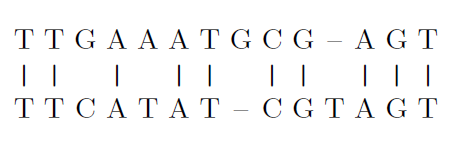
\includegraphics[width=0.5\textwidth]{fig/alignment}
    \caption{Global alignment of two DNA strings with 10 matches, two mismatches
	G/C and A/T, and two gaps G/– and –/T \cite[Figure 8.2]{gokhale_reconfigurable_2010}}
    \label{fig:alignment}
\end{figure}

The global alignment is stretched over the entire sequence whereas the local alignment limits to strong matches within
the sequence as shown in \cref{fig:localglobal}. 

\begin{figure}%
    \centering
    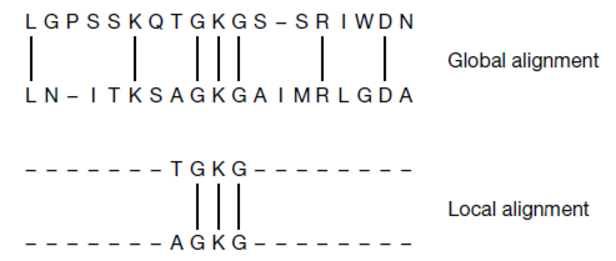
\includegraphics[width=0.6\textwidth]{fig/localglobal}
    \caption{Distinction between local and global alignment \cite[Figure 3.1]{mount_bioinformatics:_2004}}
    \label{fig:localglobal}
\end{figure}

Formally considering two string $ X = \{x_1, x_2, ..., x_n\} $ and $Y = \{y_1, y_2, .... y_n\}$
and H(i,j) maximum similarity score at position i, j, then the global alignment of the strings H(i,j) given by
the Needleman-Wunsch equation \cite{needleman_general_1970} is 

\( \forall i :  H(i,0) = g_{penalty} \times i \) \,\,\,\,\,\,\, \( \forall j :  H(0,j) = g_{penalty} \times j \)

\( \forall i,j,ij \neq 0: \)

\[ H(i,j) =  max
\begin{cases}	
	H(i - 1, j - 1) + d(x_i, y_j) & \quad \text{(match or substitution)} \\
	H(i - 1, j) - g_{penalty} 	  & \quad \text{(insertion)}\\
	H(i, j - 1) - g_{penalty}     & \quad \text{(deletion)}
\end{cases}
\]

The local similarity which is defined for the most similar pair of sub-sequences ending at $x_i$ and $y_i$ is given by
Smith-Waterman \cite{smith_identification_1981} equation as follows:

\( \forall i,j :  H(i,0) = H(0,j) = 0 \)

\( \forall i,j,ij \neq 0: \)

\[ H(i,j) =  max
\begin{cases}
	0							  & \quad \text{(local align. starts here)} \\
	H(i - 1, j - 1) + d(x_i, y_j) & \quad \text{(match or substitution)} \\
	E(i,j)	  & \quad \text{(insertion)}\\
	F(i,J)    & \quad \text{(deletion)}
\end{cases}
\]
where
\[
E(i,j) = max \begin{cases} H(i - k, j) - g_{penalty}(k), & \quad for \,\, 0 < k < i, \end{cases} 
\]
\[
F(i,j) = max \begin{cases} H(i,j - l) - g_{penalty}(l), & \quad for \,\, 0 < l < j, \end{cases}
\]

An example of both global and local alignment calculation is shown in \cref{fig:alignexample}
\begin{figure}%
    \centering
    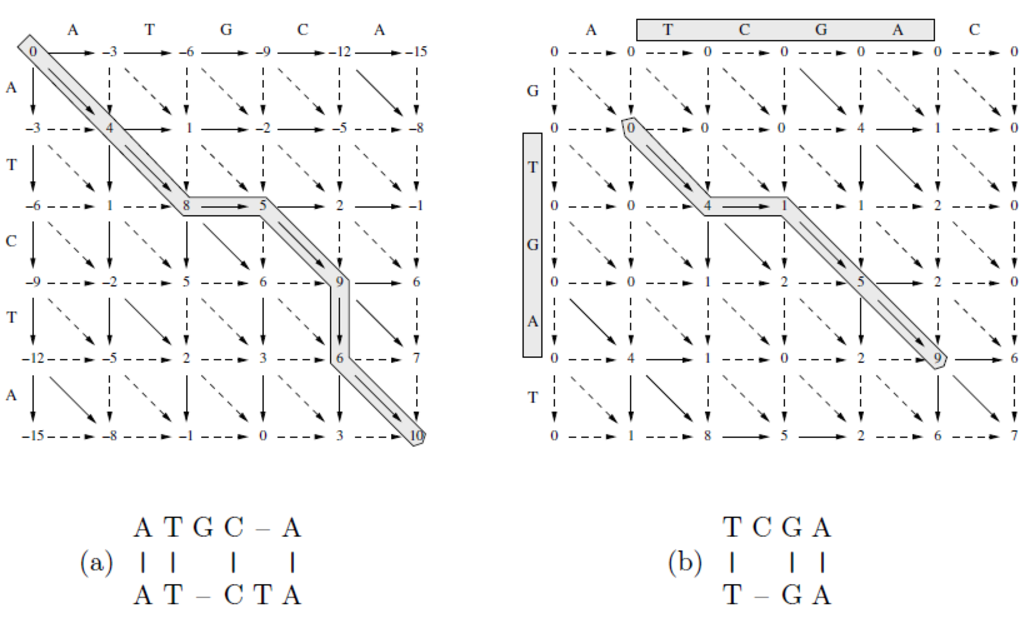
\includegraphics[width=0.9\textwidth]{fig/alignexample}
    \caption{Example of global alignment computation with the NW equation (a) and
	local alignment computation with the SW equation (b). Scores are +4 for a match,
	-2 for a mismatch, and -3 for a gap. The solid arrows are the dependencies that
	lead to the maximum of each (i, j) cell and reveal the best alignment \cite[Figure 8.4]{gokhale_reconfigurable_2010}}
    \label{fig:alignexample}
\end{figure}

\subsubsection{Seed-based Heuristics}

As highlighted in the previous sections dynamic programming algorithm are capable of performing mathematically accurate 
searches but are time consuming. This led researchers build faster algorithms which were based on some heuristics
to decrease the time of search and maintaining similar accuracy. FAST \cite{pearson_improved_1988} and BLAST \cite{altschul_basic_1990}
were initial algorithm proposed based on heuristics which performed very well.

The main idea of heuristics based algorithm is the assumption that important similarities which are small (seeds) are conserved in the same
way. This allows the algorithm to perform the dynamic programming calculations only around these seeds. BLAST like algorithm basically
execute in three stages as presented in \cite{gokhale_reconfigurable_2010}:

\begin{enumerate}
	\item Look for the exact seeds that appear in both strings.
	\item Extend each seed with a limited number of substitution. At this point no insertions or deletion is allowed.
		  The seeds whose score is greater than a defined threshold are retained.
	\item Perform full dynamic programming computation on the extended seeds.
\end{enumerate}

The stages are depicted in the \cref{fig:blastview}. The accuracy of the such algorithm depend highly on the seed size. Various extension of the algorithm has been proposed which
modify the seed selection criteria to improve the performance.

\begin{figure}[h]%
    \centering
    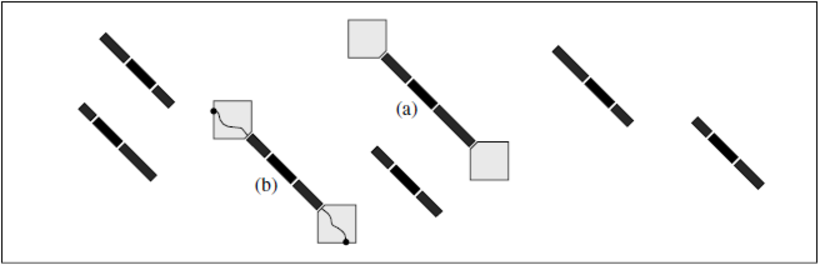
\includegraphics[width=0.8\textwidth]{fig/blastview}
    \caption{Schematic view of the BLAST 3-stages algorithm \cite[Figure 8.11]{gokhale_reconfigurable_2010}}
    \label{fig:blastview}
\end{figure}

\subsubsection{Languages Models and Profiles}

Once the a vast range of genomic strings are identified by experiments or by genome sequencing algorithms, building
a model to represent the common features among the strings is useful. As noted in previous sections, models can help
to decrease the search time of a string in databases by categorizing them based on domains. It often more helpful
to develop a generic profile which can be inferred over all the sequences.

\begin{flushleft}
\textbf{Hidden Markov Models (HMM)}: Markovian process are processes whose future states are only dependant on current state and has no effect by past states.
"HMM \cite{hughey_hidden_1996} is an statistical model which considers all the possible combination of matches, mis-matches and gaps to generate an
alignment of a set of sequences" \cite{mount_bioinformatics:_2004}. HMM needs to be trained with some initial data of known
sequences. The initial data is selected based on the family of the amino acids required to be identified. The trained HMM 
can then be used to identify sequences of the same family. \cref{fig:hmm} shows a HMM states which can be used for multiple
sequence alignment.
\end{flushleft}

\begin{figure}[h]%
    \centering
    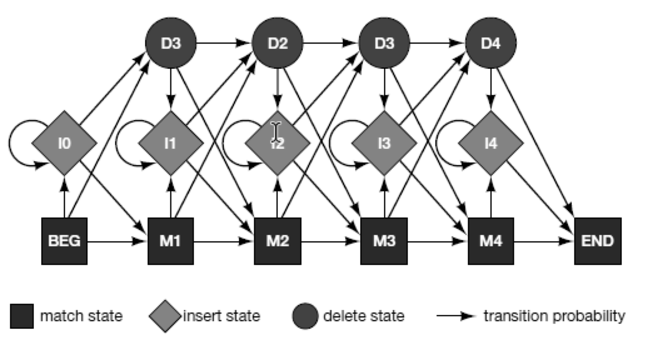
\includegraphics[width=0.8\textwidth]{fig/hmm}
    \caption{Hidden Markov model for sequence alignment \cite[Figure 4.16]{mount_bioinformatics:_2004}}
    \label{fig:hmm}
\end{figure}

\section{Optimization of Genome database search algorithms}
\label{sec:designtech}

The previous sections introduces the application areas and highlights the possibilities for using FPGA to optimize some of the application
area. This section would present a FPGA based accelerator design for the popular dynamic programming Smith-Waterman algorithm along
with the use of this accelerator in the heterogenous system to achieve faster database search.

\subsection{FPGA accelerators for Smith-Waterman}
\label{subsec:fpgaaccelerator}

The string alignment achieved by Smith-Waterman (SW) is highly dependant on the size of the search string and size of the databases.
As the size of the databases as been increasing rapidly with identification of new sequences, the processing time for the algorithm
increases similarly. As SW is very accurate and important for the bioinformatic community, various acceleration have been developed
in order to use it efficiently. Most of the acceleration achieved are done by using parallel processing. The parallelization can be achieved
by either splitting and distributing the search over multiple processors \cite{martins_multithreaded_2000, boukerche_parallel_2005, schmidt_massively_2002, rucci_smith-waterman_2014}
or by passing the database string via a systolic comparison array. The FPGA based system are used to accelerate the processing by 
building hardware systolic cells which can perform very fast comparison. In this section we look at the FPGA based systolic accelerator
designed by \textcite{oliver_hyper_2005}.

\subsubsection{Systolic cells on the FPGA platform}

Calculation presented in \cref{subsec:dp} can easily be mapped to an array of processing elements (PE) of an FPGA creating systolic cells.
Each PE can be initialized by the single character of the search string and then shift the sequence of string from the database systolically
through the array as shown in \cref{fig:systollicarray}. Considering the query string size of M and K be the size of the sequence string to be
searched, the PEs are able to complete the comparison in $ M + K-1 $ steps with M PEs instead of $ M \times K $ required for a sequential processor.

\begin{figure}[h]%
    \centering
    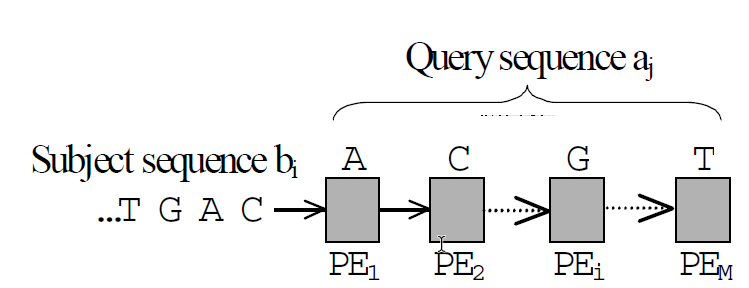
\includegraphics[width=0.7\textwidth]{fig/systollicarray}
    \caption{Systolic comparator on a linear processor array \cite[Figure 2]{oliver_hyper_2005}}
    \label{fig:systollicarray}
\end{figure}

The design presented by \textcite{oliver_hyper_2005} also utilize the reconfigurable nature of the FPGA by providing capabilities to modify the 
individual PEs to different gap penalty functions, variation of the data width (dw), substitution width (sw) and lookup address width (lw). 

\subsubsection{Operation of the cells}

Assuming a sequence query A of length M $ A = a_1a_2 .. a_M $ and B database sequence of length K $B = b_1b_2 .. b_K $ is to be mapped on a linear array of
M PEs with affine gap penalities, then during initialization $ PE i $ would be initialized with character $ a_i $ along with corresponding
gap penalities. After this the sequence B can pass through the array in $M+K-1$ steps. In each iteration k, the values H, E and F is calculated by
each PE parallely in single clock cycle. 

The above operation assume that query string size and the number of PEs are equal (M) which is not often the case. The string size will vary and 
can be greater than PE array size. In this case the computation is partitioned. Considering a query string of size M and PEs having N elements,
the query string is partitioned into $ M/N $ sequences. Initially the PEs are assigned with $ i^{th} $ partition along with gap penalities and
then the processor array goes over the database sequence iteratively. After completion of iteration the PEs are updated to next partition values.
As it is apparent, loading of the new values can be time consuming and to solve this problem the PEs are extended to store k columns of the strings along
with gap penalities to avoid memory operation. The complete system design is shown in \cref{fig:systemdesign} 

\begin{figure}[h]%
    \centering
    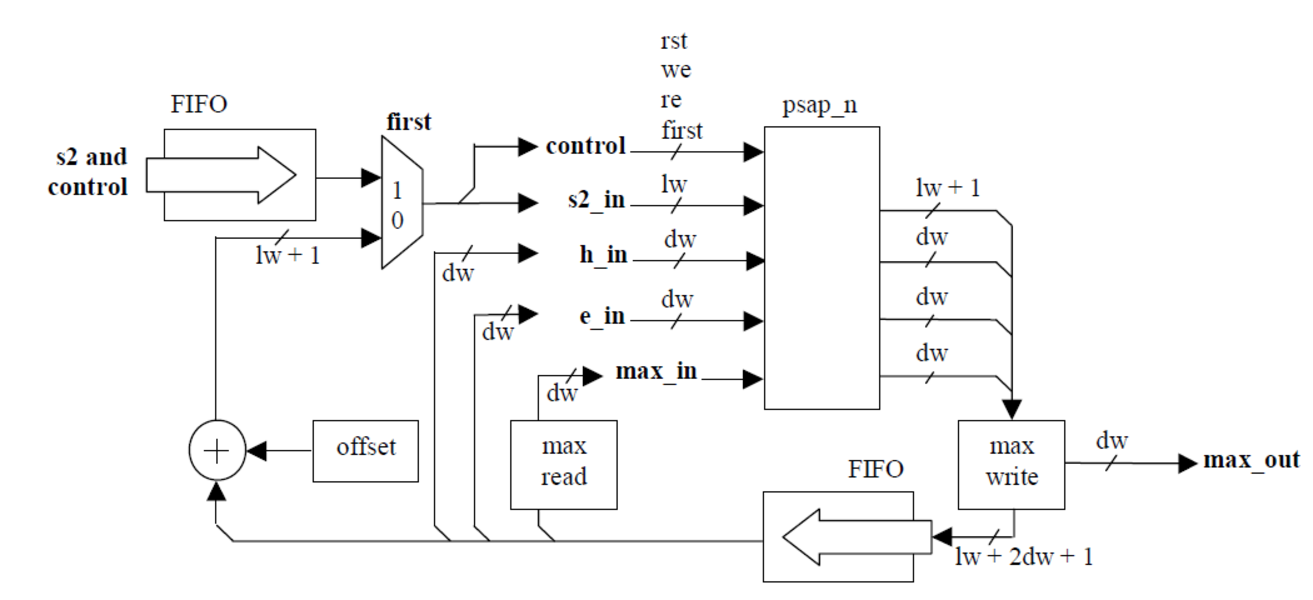
\includegraphics[width=1.0\textwidth]{fig/systemdesign}
    \caption{System design of the accelerator \cite[Figure 4]{oliver_hyper_2005}}
    \label{fig:systemdesign}
\end{figure}

\subsection{Heterogenous system design}

Using the FPGA accelerator described in the \cref{subsec:fpgaaccelerator}, \textcite{meng_high-performance_2010} implemented a heterogenous system
along with other accelerators for the Smith-Waterman algorithm which is capable of performing very fast database searches for sequence analyse.
In this section, the system would be described briefly to understand the capabilities and advantages of using a FPGA based system in a 
High performance cluster.

The system implemented by \textcite{meng_high-performance_2010} targets high speed biological sequence analysis by utilizing different accelerators
in a distributed High performance cluster environment. The target system architecture of the system is shown in \cref{fig:hetero}. The system is able
to achieve huge speed ups which will be presented in the next section. The main components of the system include SIMD calculation capable
SSE2 vector computing units, FPGA coprocessor for fast processing and legacy computer system for backward compatibility.

\begin{figure}[h]%
    \centering
    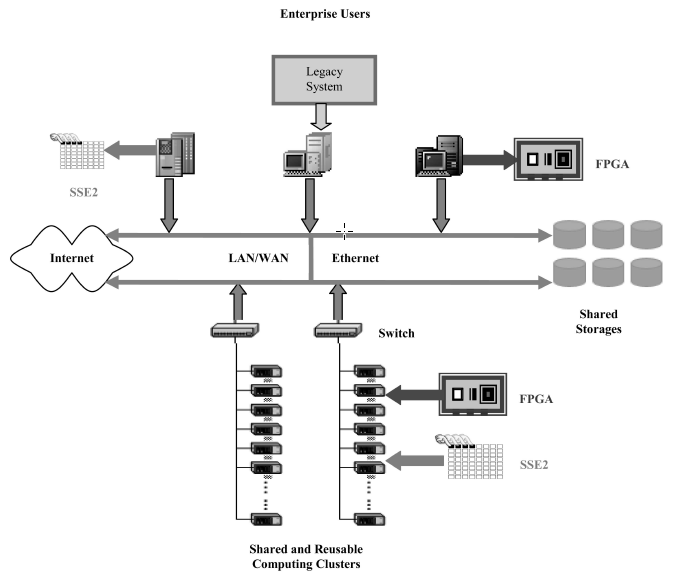
\includegraphics[width=0.8\textwidth]{fig/hetero}
    \caption{Heterogeneous computing system architecture \cite[Figure 1]{meng_high-performance_2010}}
    \label{fig:hetero}
\end{figure}

\textbf{SSE2 Vector computing} is achieved in ths system by using Intel's Pentium IV and AMD Opeteron processor capable of performing SIMD calculations
on vectors using SSE2 instruction set. This allows the nodes to perform operations on 128-bit IEEE double-precision floating data types. This is used 
to perform vector calculation to compute H, E and F by transforming the calculations to utilize SIMD operations efficiently. The minor modification in
the calculation helps to bring excellent speed up to the calculation.

\textbf{FPGA coprocessor} is integrated into the host processor. The FPGA implement the systolic array design explained in \cref{fig:systollicarray}.
To control and exchange data between host and FPGA system, board specific application interface is used. As explained the array calculates the 
similarity scores for the given query string and the database sequence and writes back them into the host memory. These flow can be used to
perform fine grained calculation on the FPGA and then using the scores to accumulate over the entire system by the host system. The mapping of the 
PEs is shown in \cref{fig:hetrosw}

\begin{figure}[h]%
    \centering
    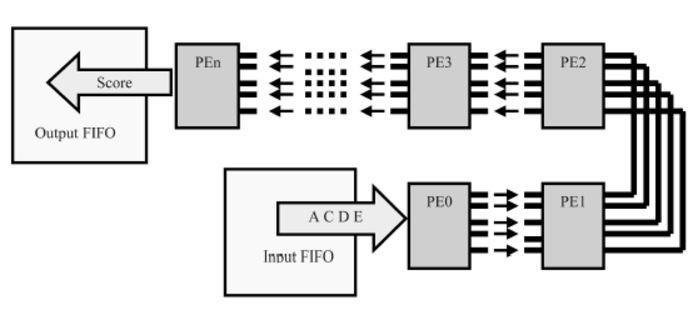
\includegraphics[width=0.6\textwidth]{fig/hetrosw}
    \caption{FPGA coprocessor mapping for linear systolic processor array \cite[Figure 3]{meng_high-performance_2010}}
    \label{fig:hetrosw}
\end{figure}

\textbf{Legacy system} are the nodes which do not support the SSE2 instruction sets. Such system are still capable of performing
sequential processing along with some software optimization. They join the computation as worker nodes and can be used to parallelize
the computation in order to utilize the full capability of the cluster.

In order to efficiently utilize the heterogenous computing resources to maximize the computation capability,
specialized scheduling and load balancing schemes were developed. The communication and control between the node is done via MPI library.
A MPI master node is used to allocate workers and distribute the workload after identification and mapping the capabilities of the node.

\section{Evaluation and comparison}
\label{sec:eval}

The evaluation of the system is essential to estimate the benefits against the cost of the system. This section will present the evaluation
strategy to estimate the performance improvement for the heterogenous system described in the previous section and highlight the major
benefits from such system.

The system was evaluated using the available genome database from NCBI and EBI. Three databases were used. First FASTA format database
containing 2,974,038 characters in 6,298 sequences. Uniref50 format containing 586,687,758 characters in
846,716 sequences and month.aa database contains 122,650 sequences and 43,531,487 characters  \cite{meng_high-performance_2010}.
Using various sources of database guarantees
the robustness of the system over variable sequence size distribution. In this evaluation only one node was equipped with FPGA co-processor
which had 119 affine PEs.
\begin{figure}[h]%
    \centering
    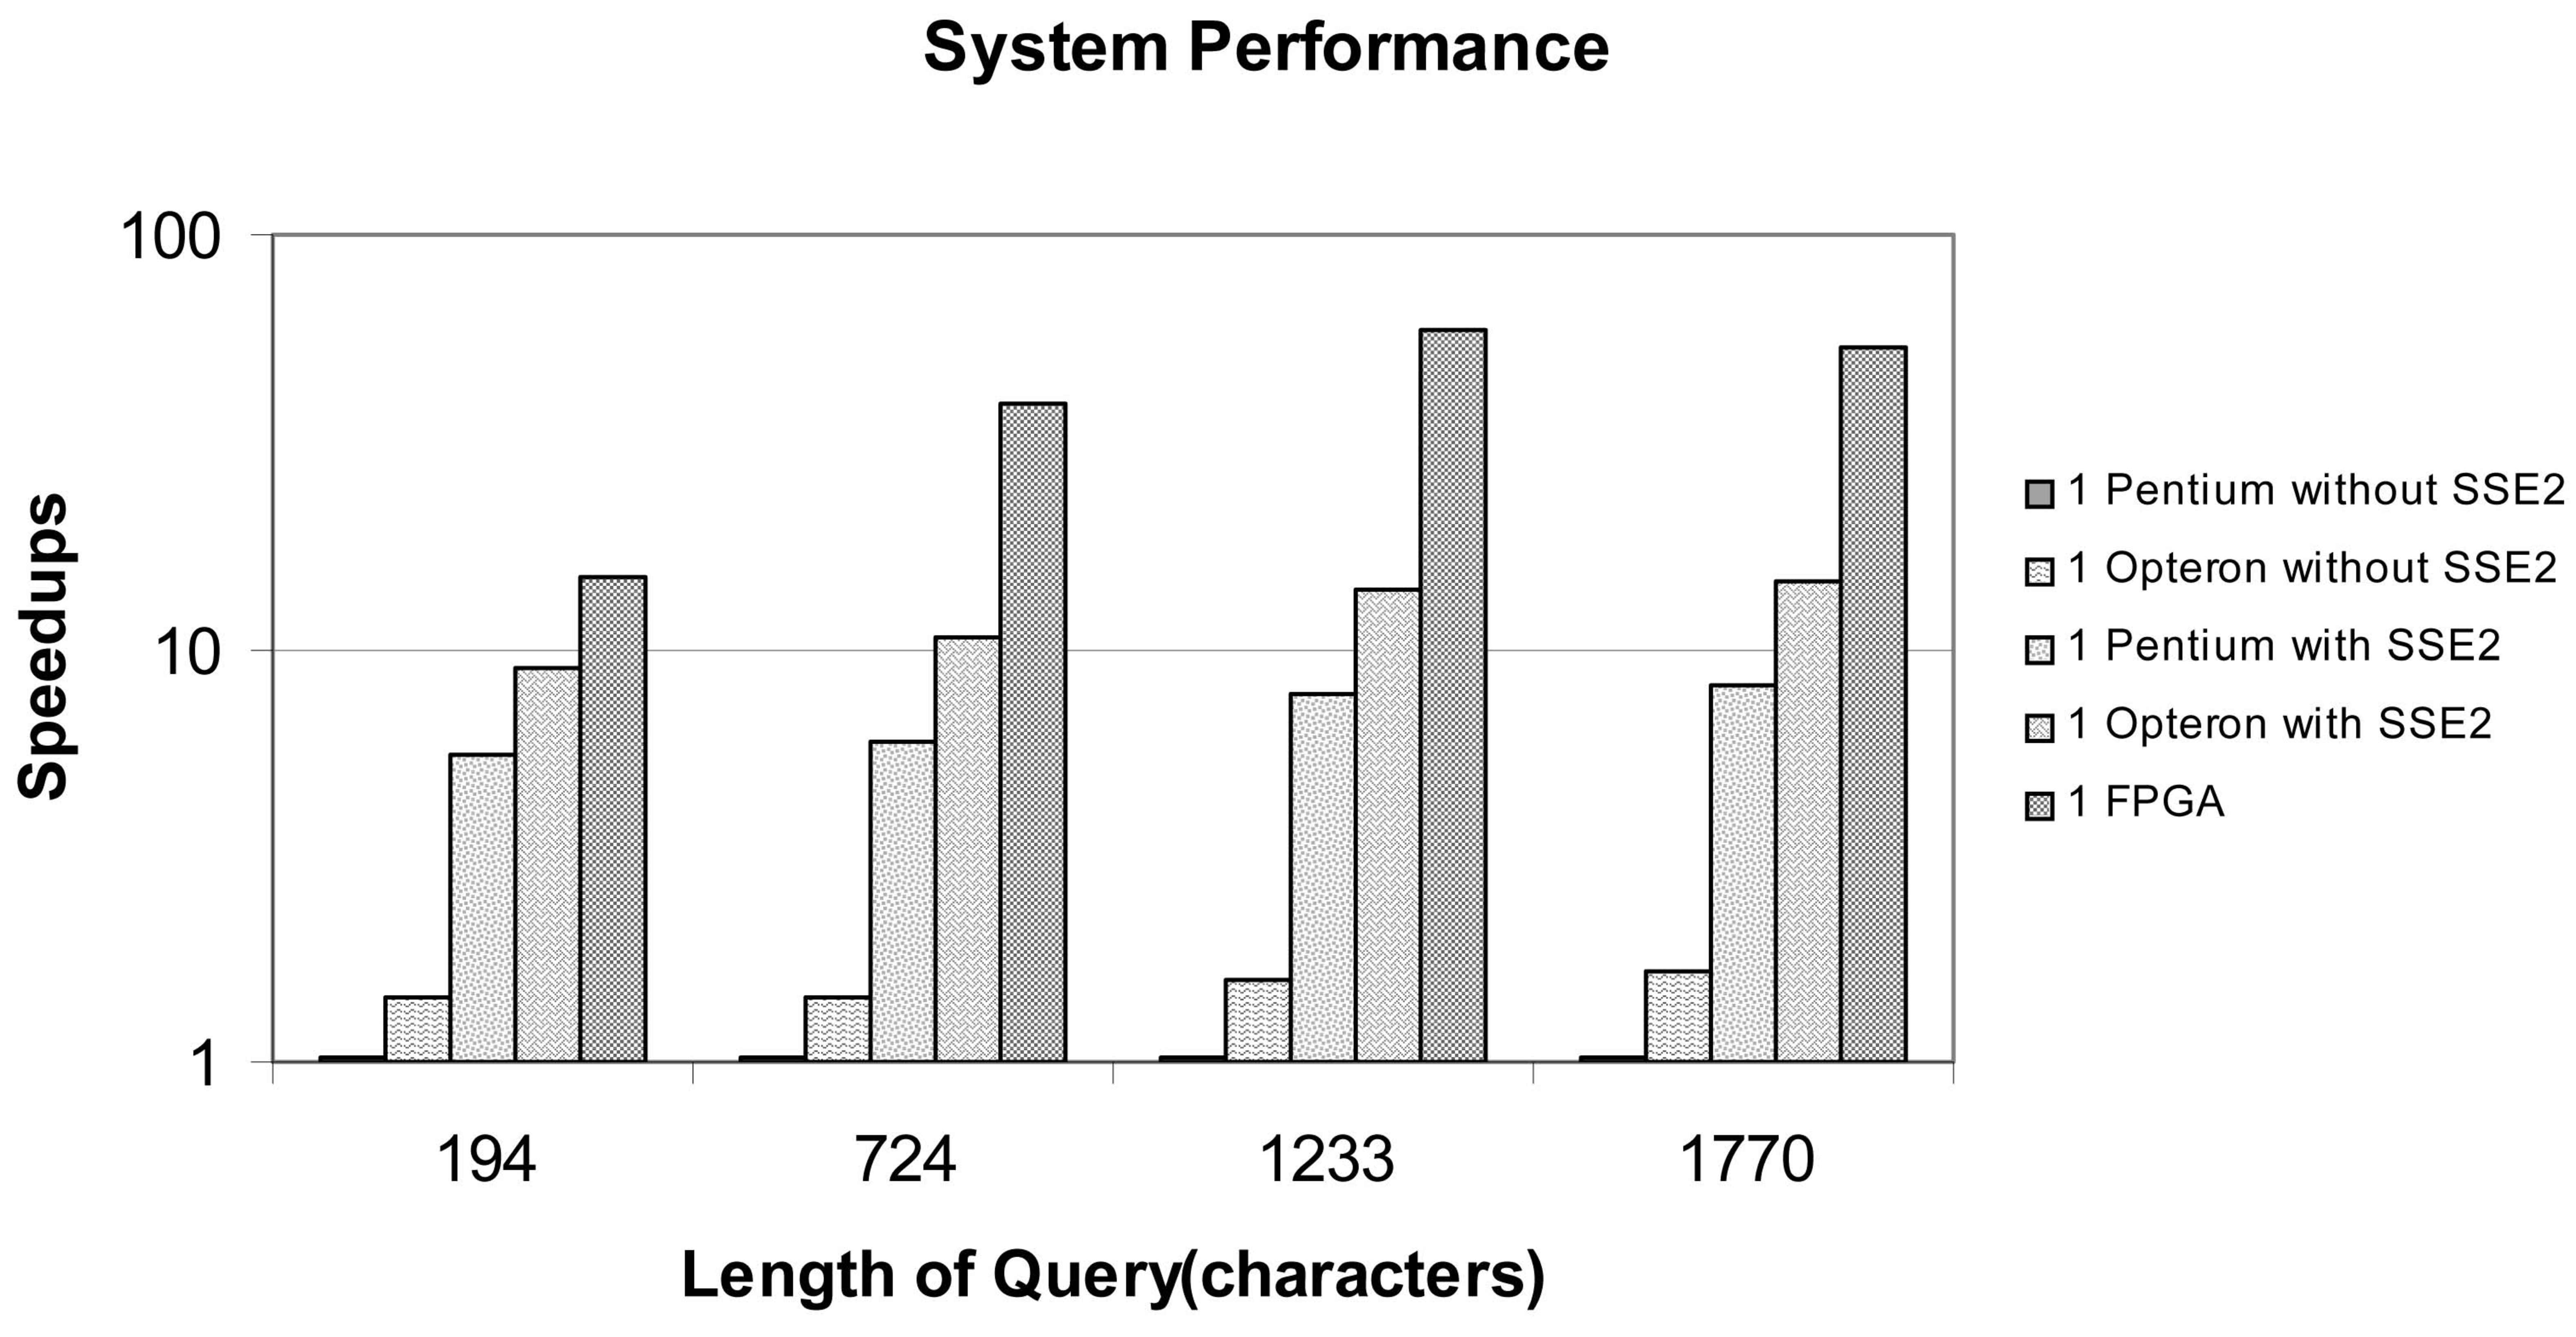
\includegraphics[width=0.8\textwidth]{fig/perform1}
    \caption{Speedup of various query lengths for various configurations \cite[Figure 10]{meng_high-performance_2010}}
    \label{fig:perform1}
\end{figure}
As shown in the \cref{fig:perform1}, a speed up of 110x is achievable with a combination of FPGA, SSE2 and MPI nodes when compared
to a serial implementation on a single Pentium IV 1.9 GHz processor. Also tests were performed to compare the speedup achieved by the 
Heterogeneous processing element compared to uniform cluster environment with multiple similar processing nodes working using MPI.
In this case as well, for the same number of nodes a 16x speed up is observed. A comparison of the speed up for a 1233 size query on month.aa and 
uniref50 database is shown in \cref{fig:perform2} to show the speed ups for different worker nodes sizes.

\begin{figure}[h]%
    \centering
    \subfloat[month.aa]{\label{fig:perform2a}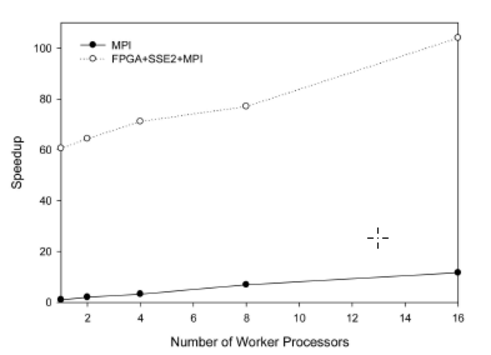
\includegraphics[width=0.5\textwidth]{fig/perform2a}}
	\subfloat[uniref50]{\label{fig:perform2b}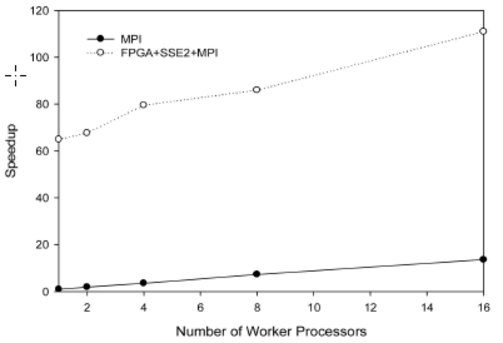
\includegraphics[width=0.5\textwidth]{fig/perform2b}}
    \caption{Performance comparison of heterogeneous \cite[Figure 12 (e,f)]{meng_high-performance_2010}}
    \label{fig:perform2}
\end{figure}

\section{Conclusion}
\label{sec:concl}

This paper introduces the various bioinformatic application and algorithm which are popular in the domain along with the optimization
which has been done by the use of FPGA and HPC system to achieve high speed up. As it is shown, a single FPGA coprocessor
posses very high potential for accelerating the algorithmic calculation required for the sequence analysis by a factors of 16. FPGA based 
acceleration has been a prime research area in the bioinformatic community and the capabilities demonstrated in this paper with a heterogeneous
system makes it very suitable for future. Various research have been carried out to accelerate other algorithms such as BLAST using
specific implementations.

Currently various organizations provide products which are based on FPGA and can be integrated in th existing HPC system to provide the additional accelerations.
\emph{Timelogic}\footnote{\url{http://www.timelogic.com/}} provides DeCypher\footnote{\url{http://www.timelogic.com/catalog/755/decypher}} suite which include
hardware accelerators for Smith-Waterman (\emph{DeCypherSW\texttrademark}), BLAST (\emph{Tera-BLAST\texttrademark}) and HMM (\emph{DeCypherHMM\texttrademark})
which can be used to accelerate the genome analysis. Similarly there are various other accelerators and projects which are aimed at integrating the FPGA coprocessor into existing HPC systems or creating new
ones to benefit from this acceleration.

Looking at such improvements, it would be possible in near future to use the genome analysis tools for analyzing data in real-time and use it to
discover therapeutic remedies for many diseases and uncover many mysteries of the human and biological world. 

%% the following commands include the biliographic information (in BibTeX format) from the
%% file template.bib

\printbibliography

\end{document}
